\chapter{الأعضاء والأدوار ونقاط البداية}
\label{ch:02-roles}
\section{من يعمل في المسح؟}
\label{sec:observatory-responsibilities}

يمر كل مسح بأيدي عدة أشخاص: أحدهم يجهّز العمل، وآخر يجمع البيانات، وغيرهم يراجعونها ثم يستخدمون نتائجها. يعرض الجدول التالي شخصيات العمل في المسح الصناعي الوطني، وما يفعله كل منها، ومن يؤديها في مثالنا.

\begin{table}[H]
\centering
\caption{شخصيات العمل في المسح ومقابلها في مثال مصنع الأفق}
\label{tab:observatory-responsibilities}
\begin{tabularx}{\linewidth}{R{2.8cm} Y R{2.6cm}}
\rcHeaderRow
\thh{الشخصية} & \thh{عملها في المسح} & \thh{في مثالنا}\\
مسؤول المؤسسة & يجهّز الحسابات والمناصب والصلاحيات وإعدادات المؤسسة. & مسؤول المؤسسة\\
مدير المسح & يبني الحزمة وخطة التكليف، ويطلق الجولة ويتابع توزيع العمل. & سارة\\
الباحث الميداني & يعبّئ النماذج لمنشآته، على الهاتف غالباً، ويرسلها ويصحّح ما يُعاد إليه. & عمر\\
قائد الفريق & يراجع كل إجابة بعد التدقيق الآلي، ثم يعتمدها أو يعيدها للتصحيح أو يرفضها. & ليلى\\
مدقق المحافظة & يضيف توقيعاً ثانياً على نماذج محددة فقط، لا على كل النماذج. & خالد، مدقق ريف دمشق\\
محلل الموضوع & يوقّع التوقيع الأخير بحسب موضوع النموذج، ويتابع لوحة جودة البيانات. & رنا\\
مدير المرصد & يقرأ لوحات المؤشرات وبيانات الجولات. & هالة\\
موظف السجل & يعدّل ملفات المنشآت وقيود السجل الصناعي. & يوسف\\
\end{tabularx}
\end{table}

قد يجمع شخص واحد أكثر من عمل، لكن قيامه بأحدها لا يمنحه الأعمال الأخرى تلقائياً؛ فلكل عمل صلاحياته الخاصة.

\begin{rcnote}[تطبيق المثال: فريق مصنع الأفق]
عرّفنا في الفصل الأول سارة وعمر وليلى. ونضيف الآن أربعة أشخاص يكملون الرحلة: خالد يوقّع توقيعاً ثانياً على «بيانات التشغيل»، ورنا توقّع التوقيع الأخير، وهالة تقرأ النتائج في اللوحات، ويوسف يتابع ملف المصنع في السجل الصناعي. كلهم أشخاص افتراضيون، ولم تُنشأ حساباتهم في النظام بعد.
\end{rcnote}

\section{كيف تنتقل الإجابة من شخص إلى آخر؟}
\label{sec:observatory-approval-path}

لا تصبح الإجابة معتمدة بمجرد إرسالها. فهي تمر بمراحل ثابتة، ولكل مرحلة شخص يقرر فيها، ولا تبدأ مرحلة حتى تنتهي التي قبلها.

\begin{figure}[H]
\centering
\begin{tikzpicture}[node distance=0.4cm,stepBox/.append style={minimum width=6cm,text width=5.6cm,minimum height=0.7cm}]
  \node[stepBox] (s0) {\RL{عمر يعبّئ النموذج}\\\RL{ويرسله}};
  \node[stepBox,below=of s0] (s1) {\RL{التدقيق الآلي يقترح}\\\RL{ولا يعتمد شيئاً}};
  \node[stepBox,below=of s1] (s2) {\RL{ليلى، قائدة الفريق}\\\RL{تعتمد أو تعيد أو ترفض}};
  \node[stepBox,below=of s2] (s3) {\RL{خالد، مدقق المحافظة}\\\RL{على «بيانات التشغيل» فقط}};
  \node[stepBox,below=of s3] (s4) {\RL{رنا، محللة الموضوع}\\\RL{التوقيع الأخير}};
  \node[stepBox,below=of s4] (s5) {\RL{الإجابة معتمدة}\\\RL{وتُكتب في ملف المصنع}};
  \draw[flowsTo] (s0) -- (s1);
  \draw[flowsTo] (s1) -- (s2);
  \draw[flowsTo] (s2) -- (s3);
  \draw[flowsTo] (s3) -- (s4);
  \draw[flowsTo] (s4) -- (s5);
\end{tikzpicture}
\caption{مسار إجابة مصنع الأفق من الإرسال إلى الاعتماد}
\label{fig:observatory-approval-path}
\shotnote{يبيّن المخطط ترتيب المراجعة الذي سنطبقه على مثالنا، وهو الترتيب نفسه المستخدم في المسح الوطني. المهم فيه أن الإجابة لا تصل إلى ملف المصنع إلا بعد آخر توقيع. أما نموذج «متابعة الاحتياج» فينتقل من ليلى إلى رنا مباشرة، لأن مرحلة المدقق تقتصر على النماذج المحددة لها.}
\end{figure}

\textbf{قواعد المسار} — تنطبق على كل نموذج في الحزمة:

\begin{enumerate}
\item \textbf{الإرسال يبدأ المراجعة:} حين يضغط الباحث «إرسال الطلب»، تبدأ «جولة الموافقة 1» تلقائياً، وتأخذ الإجابة رقمها النهائي بدل رقم المسودة.
\item \textbf{التدقيق الآلي يقترح فقط:} يقترح لكل إجابة «صحيح» أو «يحتاج تصحيحاً» مع السبب، ويترك للمراجع ما لا يستطيع الحكم عليه. القرار دائماً للمراجع.
\item \textbf{لكل مراجع ثلاثة قرارات:} «اعتماد» والتعليق فيه اختياري، و«إعادة للتصحيح» والتعليق فيها مطلوب، و«رفض» والتعليق فيه مطلوب أيضاً.
\item \textbf{التقييم يسبق القرار:} تحت كل إجابة يختار المراجع «صحيح» أو «يحتاج تصحيحاً» أو «غير منطبق». وعند اختيار «يحتاج تصحيحاً» يكتب ملاحظة تشرح للباحث ما يجب تصحيحه.
\item \textbf{لا اعتماد مع إجابة معلَّمة:} يبقى زر «اعتماد» معطلاً ما دامت هناك إجابة قيّمها المراجع «يحتاج تصحيحاً». أما اقتراحات التدقيق الآلي فلا تمنع الاعتماد.
\item \textbf{الإعادة تفتح المعلَّم فقط:} عند الإعادة تُفتح للباحث الأسئلة المعلَّمة وحدها، ويرى ملاحظة المراجع تحتها، وتبقى بقية الصفحات للعرض فقط.
\item \textbf{إعادة الإرسال تبدأ جولة جديدة:} تبدأ «جولة الموافقة 2» من التدقيق الآلي، وتُحفظ الجولة الأولى وتقييماتها في السجل.
\item \textbf{مدقق المحافظة على نماذج محددة:} في المسح الوطني يوقّع المدقق على الوحدتين الأوليين فقط. وفي مثالنا يوقّع خالد على «بيانات التشغيل» وحده.
\item \textbf{الكتابة في السجل بعد آخر توقيع:} لا تُكتب الإجابات في ملف المنشأة، ولا تظهر في اللوحات، إلا بعد الاعتماد الأخير.
\end{enumerate}

\begin{rcnote}[تطبيق المثال: رحلة إجابة عمر]
يرسل عمر «بيانات التشغيل»: 24 عاملاً، و3 أيام توقف، والسبب «أخرى». تلاحظ ليلى أن السبب غير محدد، فتقيّمه «يحتاج تصحيحاً» وتكتب: «حدّد سبب التوقف». يتعطل زر «اعتماد»، فتضغط «إعادة للتصحيح» وتكتب التعليق نفسه. يفتح عمر النموذج فيجد سؤالاً واحداً مفتوحاً، فيختار «انقطاع الكهرباء» ويرسل من جديد. تبدأ الجولة الثانية، فتعتمد ليلى، ثم خالد، ثم رنا. عندها تصبح الإجابة «معتمدة»، ويرى يوسف الأرقام في ملف المصنع، وتراها هالة في اللوحات.
\end{rcnote}

هذا هو المسار الذي سنعدّه لمثالنا عند بناء النموذج في الفصل الرابع، ثم نختبره خطوة خطوة في فصل المراجعة. تعرض الصورة التالية إجابة حقيقية أنهت هذا المسار كاملاً.

\begin{figure}[H]
\centering
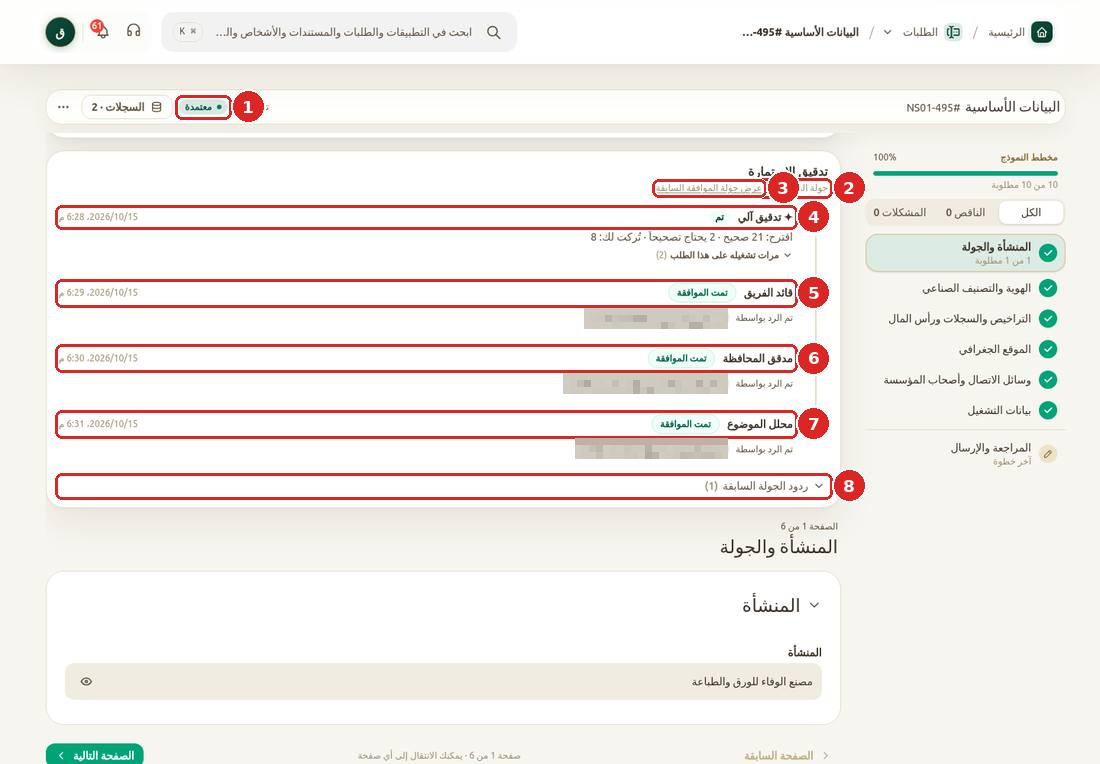
\includegraphics[width=\linewidth]{assets/screens/roles-approval-chain-ar.png}
\caption{إجابة معتمدة بعد مرورها بكل مراحل المراجعة}
\label{fig:observatory-approval-chain}
\shotnote{تعرض الصورة قسم «تدقيق الاستمارة» في إجابة اكتملت مراجعتها، وفيه كل مرحلة ووقت التوقيع عليها. تفيدك في معرفة مكان الطلب في أي لحظة، ومن ينتظر ردّه. ولاحظ أن هذه الإجابة أُعيدت مرة ثم اعتُمدت في الجولة الثانية، كما سيحدث مع إجابة عمر. ① «معتمدة»: الحالة النهائية بعد آخر توقيع. ② رقم جولة الموافقة الحالية. ③ «عرض جولة الموافقة السابقة»: لقراءة تقييمات الجولة الأولى. ④ «تدقيق آلي»: اقتراحاته وعددها. ⑤ قائد الفريق: «تمت الموافقة». ⑥ مدقق المحافظة: «تمت الموافقة». ⑦ محلل الموضوع: التوقيع الأخير. ⑧ «ردود الجولة السابقة»: الإعادة التي حدثت في الجولة الأولى.}
\end{figure}

\section{من أين يبدأ كل شخص؟}
\label{sec:observatory-starting-points}

ابدأ دائماً من العمل المطلوب منك، لا من القوائم كلها. فالباحث لا يحتاج إلى فتح محرر الحزمة، والمراجع لا يحتاج إلى لوحة الخطة كي يعتمد إجابة.

\begin{table}[H]
\centering
\caption{نقطة البداية لكل شخص}
\label{tab:observatory-starting-points}
\begin{tabularx}{\linewidth}{R{2.8cm} Y Y}
\rcHeaderRow
\thh{الشخص} & \thh{ماذا يفتح؟} & \thh{ماذا يجد؟}\\
الجميع & الصفحة الرئيسية بعد الدخول. & ملخص «بانتظارك»: طلبات الموافقة، والتكليفات المطلوبة منه، والمهام المستحقة.\\
عمر & «المهام» ثم «التكليفات». & بطاقة لكل منشأة، ونقطة لكل نموذج، وزر الإجراء التالي.\\
ليلى وخالد ورنا & «طلبات الموافقة». & «بانتظارك» لما ينتظر ردهم الآن، و«بانتظار الآخرين» لما انتقل إلى مرحلة لاحقة، و«مكتملة» لما انتهى.\\
سارة & «المهام» ثم «التكليفات» ثم «الخطط». & خطط التكليف وحالاتها: مسودة، أو نشطة، أو موقوفة، أو مغلقة.\\
هالة ورنا & تطبيق «المرصد الصناعي» ثم «لوحات المؤشرات». & اللوحات بحسب صلاحياتهما. الباحث الميداني لا يرى اللوحات.\\
يوسف & تطبيق «السجل الصناعي» ثم «المنشآت الصناعية». & ملفات المنشآت وقيودها، ومنها ملف مصنع الأفق.\\
\end{tabularx}
\end{table}

\begin{figure}[H]
\centering
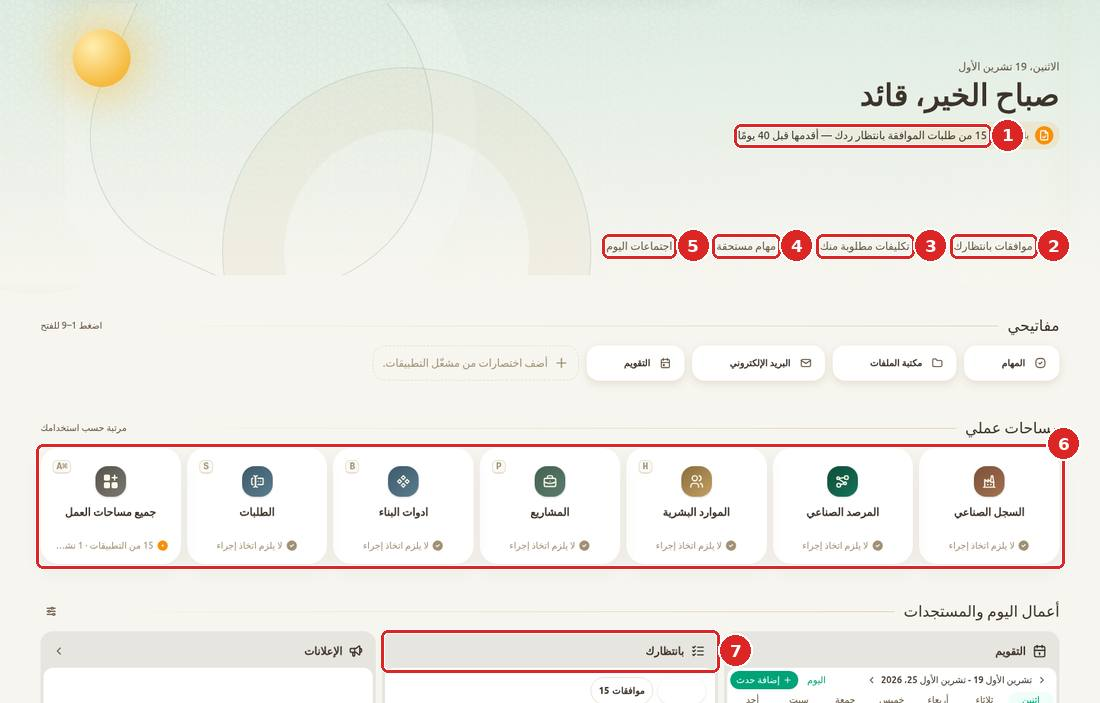
\includegraphics[width=\linewidth]{assets/screens/roles-home-leader-ar.jpg}
\caption{الصفحة الرئيسية لقائد الفريق}
\label{fig:observatory-home-leader}
\shotnote{هذه أول شاشة تراها ليلى بعد الدخول، وهي تجمع ما ينتظرها من كل التطبيقات. تفيدها في معرفة عدد طلبات الموافقة وعمر أقدمها قبل أن تبحث في أي قائمة. ابدأ من الملخص في الأعلى، ثم افتح الطلب من بطاقة «بانتظارك». ① ملخص ما ينتظرك وعمر أقدم طلب. ② «موافقات بانتظارك». ③ «تكليفات مطلوبة منك». ④ «مهام مستحقة». ⑤ «اجتماعات اليوم». ⑥ «مساحات عملي»: تحت كل مساحة ما يحتاج إجراءً فيها. ⑦ بطاقة «بانتظارك»: اضغط أي طلب لفتحه.}
\end{figure}

\begin{figure}[H]
\centering
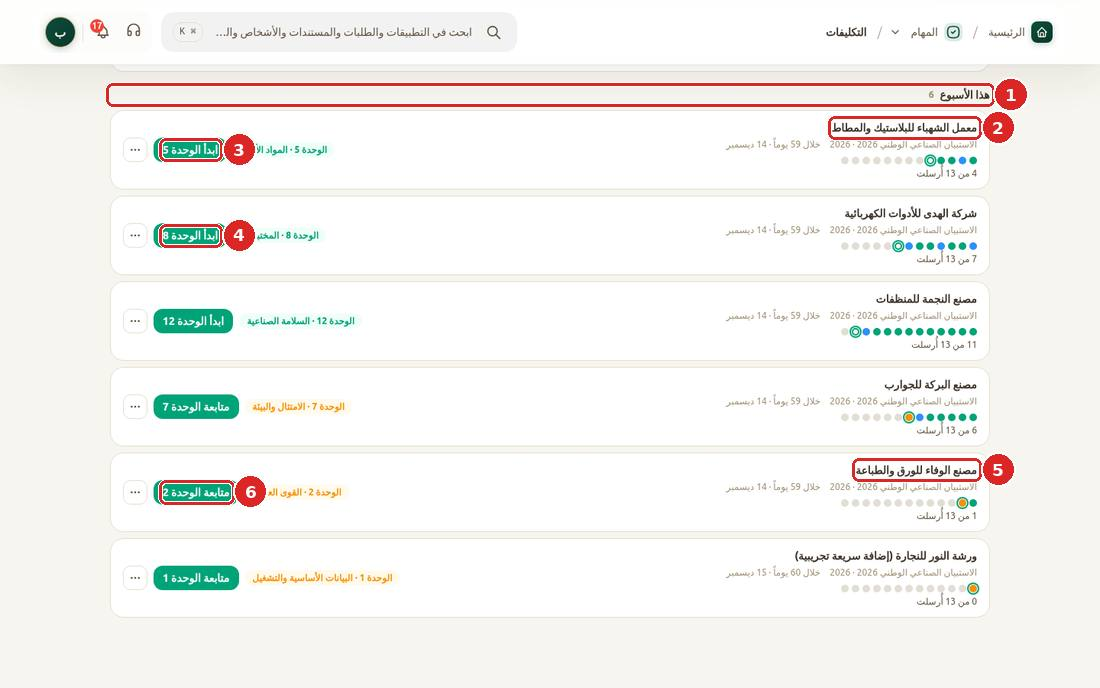
\includegraphics[width=\linewidth]{assets/screens/roles-assignments-researcher-ar.jpg}
\caption{تكليفات الباحث الميداني لهذا الأسبوع}
\label{fig:observatory-assignments-researcher}
\shotnote{هنا يبدأ عمر عمله اليومي: لكل منشأة بطاقة تبيّن موعدها وتقدّم نماذجها. تفيده النقاط الملونة في معرفة النموذج التالي دون فتح المنشأة؛ فالأخضر مقبول، والأزرق مُرسل، والبرتقالي قيد التعبئة، والأحمر بحاجة إلى تعديل، والرمادي مقفل. ويختصر زر البطاقة الخطوة التالية. ① مجموعة «هذا الأسبوع». ② اسم المنشأة، وتحته موعدها ونقاط نماذجها. ③ «ابدأ الوحدة 5»: يفتح النموذج التالي. ④ «ابدأ الوحدة 8»: نموذج يُفتح بشرط، وقد تحقق شرطه لهذه المنشأة. ⑤ منشأة اعتُمد نموذجها الأول. ⑥ «متابعة الوحدة 2»: يكمل مسودة محفوظة.}
\end{figure}

\begin{rcnote}[تطبيق المثال]
عندما نطلق خطة «متابعة تشغيل الأفق»، يجد عمر بطاقة مصنع الأفق في «التكليفات» وعليها نقطتان: «بيانات التشغيل» ثم «متابعة الاحتياج». وبعد أن يرسل، يظهر الطلب لليلى في صفحتها الرئيسية وفي «طلبات الموافقة ← بانتظارك». أما خالد فلا يرى الطلب حتى تعتمده ليلى.
\end{rcnote}

\textbf{طبّق الآن:} افتح «التكليفات» بحسابك، وانتقل بين «المطلوب مني» و«الخطط»، ثم افتح «طلبات الموافقة». حدّد أي هذه المواضع يحتوي عملك. القائمة الفارغة لا تعني وجود خطأ؛ فربما لم يصلك عمل بعد. ولا تستخدم حساب المسؤول لتفترض أن شاشة عمر أو ليلى ستظهر بالشكل نفسه.

\section{العضو والمنصب والصلاحية}
\label{sec:observatory-people-terms}

الشخصية تصف العمل الذي يؤديه الشخص. أما ما يستطيع فعله داخل النظام فيحدده أمران: موقعه في الهيكل التنظيمي، والصلاحيات الممنوحة له.

\begin{table}[H]
\centering
\caption{ثلاثة مفاهيم لا نخلط بينها}
\label{tab:observatory-people-terms}
\begin{tabularx}{\linewidth}{R{3cm} Y}
\rcHeaderRow
\thh{المفهوم} & \thh{معناه ببساطة}\\
العضو & حساب الشخص في المؤسسة. وجوده وحده لا يعطيه أي تكليف.\\
المنصب والتعيين & المنصب موقع داخل وحدة تنظيمية مثل فريق المسح، والتعيين يربط العضو بهذا المنصب. وعليهما تعتمد الخطة في اختيار الباحثين.\\
دور الصلاحيات & يحدد ما يستطيع الشخص فعله وأين. ولا يكفي اسم الدور لمعرفة ما يتيحه.\\
\end{tabularx}
\end{table}

\textbf{الصلاحيات التي يحتاج إليها المسح:} تُمنح الأعمال السابقة بأدوار صلاحيات منفصلة، منها:

\begin{itemize}
\item \textbf{فريق المسح:} قراءة المنشآت وأصولها وبيانات الجولات والقوائم المرجعية.
\item \textbf{السجل الصناعي:} تعديل المنشآت وقيودها.
\item \textbf{مراجعو المسح:} فتح إجابات النموذج وبدء مراجعتها. وتُمنح لكل نموذج على حدة.
\item \textbf{عارض لوحات المرصد الصناعي:} فتح لوحات المؤشرات.
\end{itemize}

وتوجد صلاحيات أخرى داخل الحزمة والخطة نفسيهما، ولكل منها موضعه:

\begin{table}[H]
\centering
\caption{أين نراجع كل صلاحية؟}
\label{tab:observatory-access}
\begin{tabularx}{\linewidth}{R{3cm} Y}
\rcHeaderRow
\thh{العمل} & \thh{أين نراجعه؟}\\
تعديل الحزمة ونشرها & «الوصول» في الحزمة، ثم «محررو الحزمة».\\
إدارة الخطة & «الإعداد» في الخطة، ثم «6 · من يدير الخطة» و«مسؤولو الخطة».\\
الإسناد اليدوي & «من يكلّف يدوياً ضمن الخطة». لا يمنح صاحبه إدارة النماذج.\\
مراجعة الإجابات & مسار الموافقة في النموذج، ودور «مراجعو المسح» على ذلك النموذج.\\
\end{tabularx}
\end{table}

\begin{rcnote}[تطبيق المثال]
يحتاج عمر إلى تعيين نشط في منصب «باحث ميداني» داخل «فريق مسح الأفق»، وإلى دور «فريق المسح». وتحتاج ليلى وخالد ورنا إلى دور «مراجعو المسح» على النماذج التي يراجعونها؛ فخالد يحتاجه على «بيانات التشغيل» وحده. وتحتاج هالة إلى «عارض لوحات المرصد الصناعي»، ويحتاج يوسف إلى «السجل الصناعي». ولا نحل مشكلة وصول عمر بمنحه تحرير الحزمة.
\end{rcnote}

\section{كيف تختار الخطة الباحث؟}
\label{sec:observatory-candidates}

لا تختار الخطة الباحث بالاسم، بل تتبع قاعدة. في خطة الفرق الميدانية تقرأ الخطة حقل «فريق المسح» في ملف المنشأة، ثم تبحث داخل ذلك الفريق عن شاغلي منصب «باحث ميداني - RES». بعدها تختار من بينهم بقواعد التوزيع.

\begin{figure}[H]
\centering
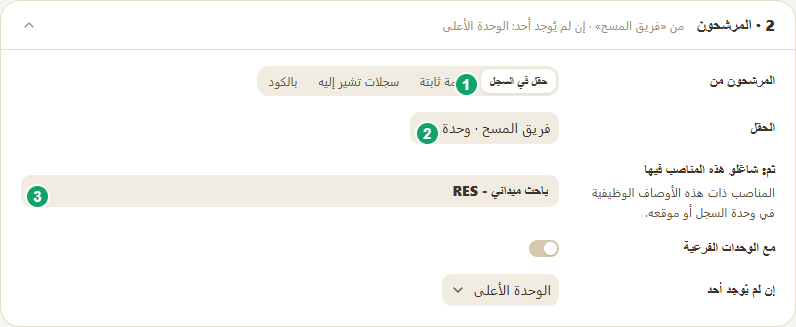
\includegraphics[width=\linewidth]{assets/screens/roles-candidates-ar.png}
\caption{مصدر المرشحين في خطة الفرق الميدانية}
\label{fig:observatory-candidates}
\shotnote{تعرض الصورة القسم الذي يحدد من أين تأتي الخطة بالمرشحين. تفيدك عندما لا يصل التكليف إلى الباحث المتوقع، لأنها تبيّن البيانات التي يجب أن تكون صحيحة: فريق المنشأة، ومنصب الباحث داخله. ① «حقل في السجل»: تأخذ الخطة المرشحين من حقل في ملف المنشأة. ② «فريق المسح · وحدة»: الحقل الذي يحدد الفريق. ③ «باحث ميداني - RES»: المنصب المطلوب داخل الفريق.}
\end{figure}

\textbf{قواعد التوزيع في خطة المسح الوطني:}

\begin{enumerate}
\item \textbf{شخص واحد لكل منشأة،} ويُختار الأقل حِملاً بين المرشحين.
\item \textbf{حد أقصى 15 منشأة لكل باحث.} من بلغ الحد لا يُكلَّف بالمزيد.
\item \textbf{نفس الشخص في الجولة التالية،} حتى يبقى الباحث الذي يعرف المنشأة.
\item \textbf{تخطّي الغائبين:} من أعلن غيابه بزر «غائب حتى…» لا يُكلَّف خلال غيابه.
\item \textbf{إن لم يوجد أحد في الفريق،} يُرفع البحث إلى الوحدة الأعلى.
\end{enumerate}

\begin{rcnote}[تطبيق المثال]
ليصل تكليف مصنع الأفق إلى عمر، يجب أن يحمل ملف المصنع «فريق مسح الأفق» في حقل «فريق المسح»، وأن يشغل عمر منصب «باحث ميداني - RES» في هذا الفريق. وحتى لو تحقق ذلك، قد لا يصله التكليف إن كان لديه 15 منشأة، أو أعلن غيابه. سنضبط قيم خطتنا عند إعدادها في الفصل الخامس.
\end{rcnote}

\textbf{افحص الإعداد دون تغييره:} بحساب مخوّل بإدارة الخطة، افتح «المهام» ثم «التكليفات» ثم «الخطط»، وافتح خطة مسموحاً لك بمراجعتها. من «الإعداد» افتح «2 · المرشحون»، واقرأ مصدر المرشحين والحقل والمنصب كما في الصورة. لا تضغط «حفظ» أو «تشغيل جولة جديدة» في هذا التمرين.

\section{إذا لم يظهر العمل، ماذا تراجع؟}
\label{sec:observatory-role-check}

حدّد المشكلة أولاً، ثم راجع موضعها. فمنح صلاحيات واسعة لا يصلح بيانات ترشيح ناقصة.

\begin{table}[H]
\centering
\caption{المشكلة وما تراجعه}
\label{tab:observatory-role-check}
\begin{tabularx}{\linewidth}{Y Y}
\rcHeaderRow
\thh{ما الذي لاحظته؟} & \thh{ما الذي تراجعه؟}\\
لا أرى «المرصد الصناعي» أو لوحاته & تأكد من اسم المؤسسة أعلى الصفحة الرئيسية. اللوحات متاحة لمدير المرصد ومحلل الموضوع ومسؤول المؤسسة فقط.\\
لا يوجد تكليف للمنشأة & نطاق الخطة وحالتها وجولتها: هل أُطلقت؟ وهل تطابق المنشأة شروطها؟\\
لا يوجد مرشح متوقع & حقل «فريق المسح» في ملف المنشأة، ومنصب الباحث وتعيينه النشط.\\
المرشح موجود ولم يُكلَّف & الحد الأقصى، والغياب، والإسناد القائم. فالترشيح لا يضمن الاختيار.\\
لا يُفتح النموذج التالي & أرسل النموذج الحالي أولاً؛ فالنماذج تُفتح بالترتيب. وقد يُفتح بعضها بشرط فقط.\\
زر «إرسال الطلب» لا يعمل & افتح «المراجعة والإرسال»، وعالج ما يظهر في «يجب معالجته قبل الإرسال».\\
زر «اعتماد» معطّل & هناك إجابة قيّمتها «يحتاج تصحيحاً». غيّر التقييم، أو أعد الطلب للتصحيح، أو ارفضه.\\
الطلب لم يصل إلى المراجع & هل انتهت المرحلة السابقة؟ فخالد لا يرى الطلب قبل اعتماد ليلى.\\
\end{tabularx}
\end{table}

\begin{rcnote}[تطبيق المثال]
إذا لم يرَ عمر مصنع الأفق، تتحقق سارة أولاً من وجود التكليف ومن أُسند إليه. وإذا لم يجد النظام مرشحاً، تراجع فريق المصنع ومنصب عمر. وإذا سيغيب عمر أسبوعاً، يضغط «غائب حتى…» في «التكليفات»، فتتخطاه الخطة، وتستطيع سارة نقل تكليفاته إلى زميل من تبويب «الفريق».
\end{rcnote}

\begin{rcchecklist}[بطاقة جاهزية فريق المثال]
\begin{checklist}
\item أعرف عمل كل شخص في فريق مصنع الأفق: سارة وعمر وليلى وخالد ورنا وهالة ويوسف.
\item أستطيع ترتيب مسار الإجابة: إرسال، ثم تدقيق آلي، ثم قائد الفريق، ثم المدقق عند الحاجة، ثم المحلل.
\item أعرف أن «إعادة للتصحيح» و«رفض» يحتاجان إلى تعليق، وأن «اعتماد» يتعطل مع أي إجابة معلَّمة.
\item أعرف نقطة البداية لكل شخص: «التكليفات» أو «طلبات الموافقة» أو «الخطط» أو اللوحات أو السجل.
\item أميّز بين المنصب الذي تختار به الخطة الباحث، والصلاحية التي تسمح له بالعمل.
\end{checklist}
\end{rcchecklist}

بهذه البطاقة نعرف من سيعمل على المسح، وكيف تنتقل الإجابة بينهم. في الفصل~\ref{ch:03-register} نجهّز ملف مصنع الأفق الذي ستستهدفه الخطة، ثم نستخدم الفريق نفسه في بقية الدليل.
